
\chapter{Skin Statistics}\label{sec:ChapSkin}
\epstopdfsetup{outdir=Chapter3/Figs/PDF/}
\ifpdf
    \graphicspath{{Chapter3/Figs/Raster/}{Chapter3/Figs/PDF/}{Chapter3/Figs/}}
\else
    \graphicspath{{Chapter3/Figs/Vector/}{Chapter3/Figs/}}
\fi


<Intro here>

\section{Chromatic Target Model}

Essentially we are looking for monochromatic objects with a small variation around an average color. Chromatic skin statistics have been collected by several authors <ref papers here> using a variety of different approaches, but most have found that the statistics are well-described by 2D Gaussians. The goal of this chapter is to find a value of $\sigma$ (two standard deviations); $\mu$, the position for the mean; and $\theta^\prime$, the angle of the major axis of the 2D Gaussian found in the LCaCb $\theta = 0$ color space. This will allow us to use the methods presented in chapter 2 to design a bespoke color space which will preserve all the chromatic information about the target model.

\section{iPhone Camera Characteristics} \label{sec:iPhoneCameraCharacteristics}

Unlike more general cameras, the iPhone's camera performs certain pre-processing tasks on the raw image before it reaches the AP layer. Typically, cameras have a specific white point value, which is the value corresponding to white. It isn't necessarily the corner of the RGB cube; finding this value is part of the camera calibration. It also determines the orientation of the luminosity axis, which passes through zero to the white point. This is why all pre-defined color space functions have an implicit white point correction. However, the iPhone's white point is always set to the corner of the RGB cube before the image reaches the AP layer. So, when developing an algorithm for the iPhone, white point correction is not necessary, while on other devices the algorithm may need to be adapted accordingly.

\begin{figure}[h!]
  \centering
    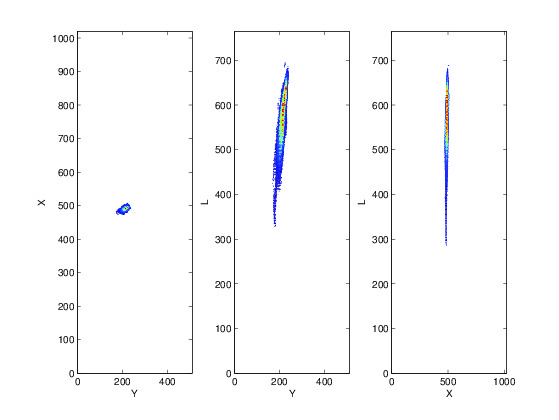
\includegraphics[width=0.80\textwidth]{Chapter3/Figs/lxy_general_white_point.jpg}
    \caption{The white point for the general skin sample set described in Section~\ref{sec:SkinStatistics}.}  \label{fig:WhitePoint}
\end{figure}

While gathering skin statistics for the purposes of this project, the original approach involved taking photos of individual skin --- each with distinct color characteristics --- taken under different lighting conditions with a constant background using the iPhone camera. The background was included in order to obtain data on the edges of the skin. The background would be photographed, then again with each individual's hand over the same background. Afterward, the statistics would be collected and the background removed by negating the background statistics.

Surprisingly, this approached failed to work; the background reappeared (Figure~\ref{fig:BGFailure}).

\begin{figure}[h!]
  \centering
    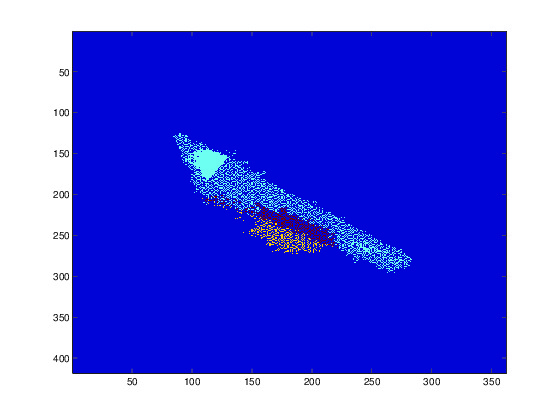
\includegraphics[width=0.60\textwidth]{Chapter3/Figs/xy_bg_failed.jpg}
    \caption{Initial attempt at removing background; unsuccessful.} \label{fig:BGFailure}
\end{figure}

The background statistics changed with the skin present in the photo. This is because the iPhone adjusts to images with very strong color characteristics. This is an undocumented feature of the iPhone processing. The only way to compensate for this unwelcome pre-processing is to photograph the background with a strongly contrasting object present, but one which is easily cropped out of the image before the background stats are collected. After collecting the statistics again, the result was much improved (Figure~\ref{fig:BGSuccess}).

\begin{figure}[h!]
  \centering
    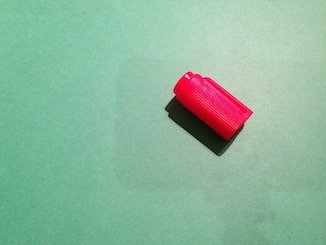
\includegraphics[width=0.60\textwidth]{Chapter3/Figs/bg_cap.jpg}
    \caption{The red marker cap contrasts with the green background.}  \label{fig:BGCap}
\end{figure}

\begin{figure}[h!]
  \centering
    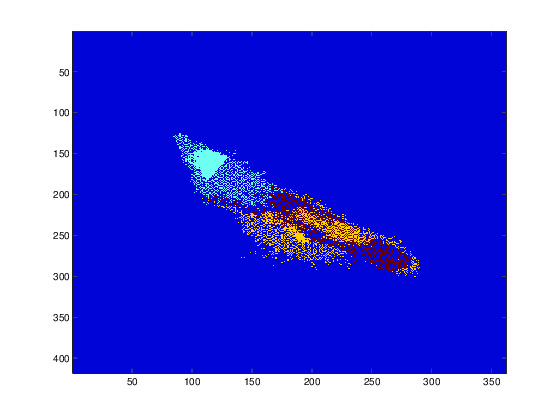
\includegraphics[width=0.60\textwidth]{Chapter3/Figs/xy_bg_success.jpg}
    \caption{Successful background removal.}  \label{fig:BGSuccess}
\end{figure}

In a real world context, it is relatively safe to presume that the scene will be chromatically complex enough that the color correction won't be detrimental to detection, and perhaps even beneficial under unusual lighting conditions. But for gathering statistics, it proved to be a massive pain.


\section{Algorithm for Generating the Model}\label{sec:AlgorithmForGeneratingModel}
Here we present the algorithm which is used to generate the chromatic model. It's assumed we have RGB image sets for the target with simple, monochromatic backgrounds.

%\animategraphics[loop,autoplay,controls]{12}{Chapter3/Figs/Animation/frame}{0001}{0025}

%\includemedia[
%  label=cube_test,
%  width=0.7\linewidth,height=0.7\linewidth,
%  addresource=Chapter3/Figs/Animation/RGB_FSkin_Hand_Bin.swf, %two video files
%  transparent,
%  activate=pageopen,
%  flashvars={
%    source=Chapter3/Figs/Animation/RGB_FSkin_Hand_Bin.swf
%   &loop=true
%   &scaleMode=letterbox
%  }
%]{}{Chapter3/Figs/Animation/RGB_FSkin_Hand_Bin.swf}


\subsection{RGB Bin Allocation}\label{sec:RGBBinAllocation}
All the information which is present in the 8-bit unsigned images is in an RGB space. The first problem is that we have a large image set with large images. We're not interested in what these images are pictures of; we're only interested in the individual pixel values themselves. So, we produce a 3D histogram with one bin for each RGB combination. This gives us a histogram with 256x256x256 bins. This is a very large data set, perhaps unnecessarily so, but it's easier to work with than a set of images and is guaranteed to contain all the relevant information for the statistics.

<put bin figure here>

The algorithm is written in MATLAB, and it very simply loads up each image in the set and runs through each pixel, incrementing the corresponding bin. As it's going, it keeps a count of the number of bin allocations, so we have a total pixel count. After it's run through all the images, it find the largest bin and keeps a record of the largest bin count, so we can have a normalized bin when requested.


\subsection{Skinning the Bins}\label{sec:SkinningTheBins}
Next, the bins which are at the extreme edges (i.e. the ones which correspond to the outer faces of the RGB cube) are set equal to 0 with a specified depth. For example: if a depth of 3 is requested, bins of positions 0, 1 and 2, and 253, 254 and 255 are set to 0 in all three dimensions, and the total pixel count is adjusted to compensate for the nulled bin counts. This is done to address problems of white-out and black-out as described in \ref{sec:TopAndTail}.

<Skinning bins figure here>

It should be noted that the reason the RGB cube is skinned before rotation is because it's not as easy to do in the rotated color space.


\subsection{Rotating the Bins}\label{sec:RotatingTheBins}
Because each of the bins corresponds to just one RGB value, we can find the equivalent bin in the LCaCb space simply by rotating the bin index. This is done using the normalized rotation as described in Chapter 2, as we desire the mean $\mu$ and standard deviation $\sigma$ to be specified in the $0:1$ range, which is easier to find where all the axes are of the same length. With this done, we now have a set of bins in the LCaCb color space equivalent to that which would be found if we had applied the transform to each of the images and then collected the statistics from the transformed images.

<Rotated bins figure here>


\subsection{Top and Tail}\label{sec:TopAndTail}

Naively collapsing the bins along the luminosity axis artificially skews the chromatic distribution along the axis which passed through the luminosity axis; this is easily explained due to white-out and black-out. As luminosity increases or decreases, it will eventually hit the edge of the cube. Having reached its numerical limit, the luminosity slides toward the corner of the cube, resulting in a white or black value.

Although we've "skinned" the bins, the white and black tips of the cube suffer from white-out and black-out more than any other regions, and there's a tendency for pixel values to converge under the white point and the black point without necessarily hitting the side of the cube first. This can be seen in <insert reference to banana picture>. There's also quite a lot of white and quite a lot of black in pretty much any image. Since we're just interested in the chromatic information, we nullify bin values above and below a certain threshold.

To accommodate this, we collapse the bins excluding the bins which are clearly suffering from white-out and black-out. This could be done mathematically by taking the bin of the distribution which is furthest from the luminosity axis, and then finding the intersection with the RGB cube when this chromatic value is at its limits, just before it reaches the edge of the cube where it suffers from white-out or black-out. But it's a simple matter to look at the three projections of the 3D LCaCb bins and manually determine the limits for the valid region.


\subsection{Collapsing the Bins}\label{sec:CollapsingTheBins}
Because we're modelling the chromatic space and not the luminosity, we now collapse the 3D histogram by summing the bin values along the luminosity axis. So, we now have a 2D histogram in CaCb chromatic space.

<figure of 3D histogram 'cause it's quite a nice thing>


\subsection{De-Speckling the Bin Values}\label{sec:DeSpeckle}
The raw camera output has, by this stage, undergone two rounds of processing --- first in the device, before the AP layer, creating an 8-bit RGB image; and then in the rotation to the LCaCb space. These processes are, unfortunately, not 1-to-1. This results in some bins being artificially overpopulated and other bins becoming artificially empty. The effect of the LCaCb rotation can be controlled by extending the axis lengths; this process can make for at worst 1-to-1 correspondence. However, this necessarily introduces a greater number of inaccessible bins. In terms of collecting the statistics, these effects are not problematic aside from the fact that it introduces empty bins inside the main region of interest, which causes difficulties for the algorithm further down the line. Graphically, this problem looks like speckling. This speckling is also apparent in the RGB bins, and it is assumed this is a result of the pre-processing of the image by the device before the AP layer. It is noteworthy that although the camera claims to capture full 3-channel, 8-bit RGB information this is not quite true. 

In attempting to solve this problem, the obvious idea is to find all the non-zero bins and fit an interpolating function between them. This will effectively remove the empty bin artefacts within the densely-packed region which is the distribution we're interested in. However, the empty bins outside the main distribution are not artefacts and are genuinely empty bins, so removing all the empty bins and then fitting the function joins together any outlying points or secondary distributions corresponding to regions such as the background. We therefore desire a method which will allow us to keep all the non-empty bins and the empty bins outside the main distribution, i.e. all the genuinely empty bins. To achieve this, we designed a Matlab routine which essentially paints a region around each non-zero point, marking it as part of the main distribution. It then takes all the unmarked regions and includes all the empty bins in those regions. So, the set of points which is all the non-empty bins and all the empty bins in the unmarked regions satisfies the requirement, and a simple interpolating function can easily be fitted to those points.

<nice little despeckling figure!>


\subsection{Blob Detection}\label{sec:BlobDetection}
Using MATLAB's blob detection algorithm, we can find the patches of chromatic information, which gives us starting values for the standard deviation. We expect there to be two distinct blobs still present: one corresponding to the target, and one to the background --- the background essentially being monochromatic. Steps 1 to 6 have also been followed for background images. 

<Insert background removal section here.>
Having removed the empty bin artefacts and compensated for white-out/black-out effects, the final step is to remove the bin counts of the bins which are associated with the background, thereby leaving a distribution which corresponds to chromatic skin values and which is artefact and systematic-error-free. With the chromatic bins processed as they have been so far, it is clear that there is a distinct distribution for the skin and a distinct distribution for the background. However, a distribution for the background was produced earlier, compensating for the iPhone's pre-AP-layer processing. Background removal is automated using a Matlab function which will negate the bins from one sample set using the distribution found for a second sample set.

<blob detection figs!>


This allows us to identify which blobs apply to the background, and sweep it clean.


\subsection{The Gaussian Fit}\label{sec:TheGaussianFit}
We now have a histogram which has bin values relevant to the target and no others. We now fit a 2D Gaussian to a normalized histogram values, initializing the routine with the values for the mean $\mu$ and the rough elliptical axis lengths for the standard deviation $\sigma$ provided by the blob detection.

<Insert bit where we copy over the angle here.>  

\begin{figure}[h!]
  \centering
    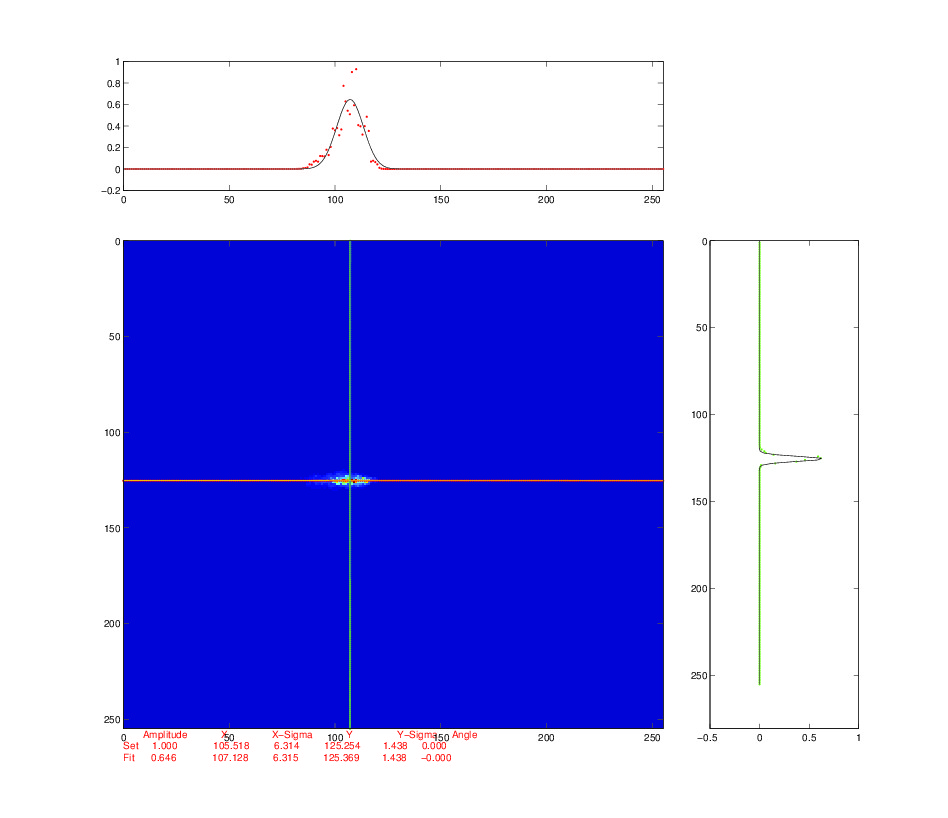
\includegraphics[width=\textwidth]{Chapter3/Figs/crosshairFigureFinal.jpg}
    \caption{Distribution and Gaussian fit to the chromatic pixel values in the new color space.}  \label{fig:DistributionAndGaussianFit}
\end{figure}

<new Mathematica figure here>

\section{Sample Sets}\label{sec:SampleSets}
There are three individual sets with different skin tones.



The MATLAB bin class was written so that the combined statistics for the three individuals could be found by adding the RGB bins together, and then following the same steps 1-8 as described previously.

<thumbnail collection here>

<table with angle theta, SD and mean for each of the three>



In order to identify the range of values for the skin space, a large number of skin samples were taken from photographs from the Humane project by Angelica Dass, an ongoing "chromatic inventory" art project which aims to compile every possible human skin color, categorized by the PANTONE guide color classification system~\cite{Dass2012}. The skin colors catalogued thus far are independent of race or ethnicity, so the samples are representative of human skin tones in general.

The image set consists of approximately 200 skin samples --- each of which shows only skin --- which are placed in a single directory in the file system. In accordance to our assumption that luminosity is not a significant factor in our skin model, we then perform the transformation initially with the value of $\theta$ equal to 0. The Matlab code collects frequency data for the rotated color space, incrementing the counts of a three-dimensional array of bins which span the color space. Viewing the frequency data along each of the three axes reveals that the skin image characteristics are spread widely in luminosity, but are quite confined in hue and saturation as illustrated in Figure~\ref{fig:InitBins}.


\begin{figure}[h!]
  \centering
    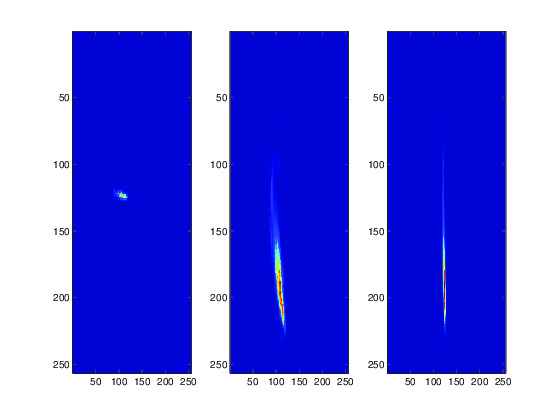
\includegraphics[width=\textwidth]{Chapter3/Figs/InitialBins.jpg}
    \caption{Initial set of bins.}  \label{fig:InitBins}
\end{figure}


Aside from differing lighting, this is consistent with the notion that skin has a distinct pigmentation and justifies our attempt to find an appropriate color space disregarding luminosity. In doing so, the distribution of the skin color characteristics neatly fit into a 2-dimensional Gaussian distribution. The Matlab code produces a fit with a 2-dimensional Gaussian distribution and provides an angle relative to the orientation of the Gaussian fit to the skin sample distribution in the current color space.

Given that we are free to choose the orientation of the color space about the luminosity axis, the Matlab code allows us to find an orientation $\theta$ of the color space about the luminosity axis in which the distribution can be expressed as a product of 1-dimensional Gaussians along the axes. The final resulting distribution is presented in Figure~\ref{fig:DistributionAndGaussianFit}.

For numerical reasons, the value for $\theta$ was found iteratively by performing the color space transformation and the statistical fit until the value for $\theta$ converged. (See Figure~\ref{fig:ConvergenceTheta}.)


\section{Implementation of Skin Color Space Statistics in Matlab}\label{sec:SkinColorSpaceStatsMatlab}

A naive approach is to take a directory of images and process them using our color space transformation with the free angle $\theta$, processing them into three-dimensional pixel value bins. It was discovered that the region of interest is relatively small in this 3D space, so it was made possible the use of a bin of width greater than 1 lumio-chromatic value. However, it is quickly found that the region of interest is so small that using a more encompassing lumio-chromatic bin is actually detrimental to the numerics involved in finding and appropriate Gaussian fit, so a lumio-chromatic bin of width 1 is used.

Because the region is so small, when the transformation is applied, we must also retain all the information therein. Initially, we did not know this; our transformed images were represented as the same data type as the original. But because the transformed information is a less efficient representation of the original information, a significant amount of that information is lost.

\begin{figure}[h!]
  \centering
    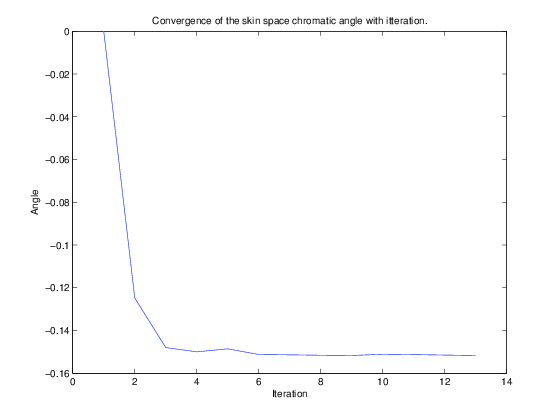
\includegraphics[width=\textwidth]{Chapter3/Figs/ConvergenceOfSkinSpaceFinal.jpg}
    \caption{Convergence of color space orientation $\theta$.}  \label{fig:ConvergenceTheta}
\end{figure}

A better approach would be to iterate over the free angle $\theta$ of the Gaussian fit of the two-dimensional bin, which was found by collapsing the 3D bins along the luminosity axis, until convergence; at best, convergence was achieved after 3 iterations. Unfortunately, this approach --- though conceptually straightforward --- is very wasteful; all of the necessary information can be found in the RGB bin statistics.

Given that we are unable to apply this process in a reasonably efficient manner to individuals and general samples, if this project is to be finished sometime this century, a more nuanced approach is necessary.

\subsection{Transformation with Zero Angle}\label{sec:TransWithZeroAngle}

The more interpretable statistics for this project is a set of bins which contains all the information in the RGB bins, but is oriented such that there is a luminosity axis and two chromatic axes. Although the rotation matrices aren't unique, a set can be chosen and an angle $\theta$ determined in the chromatic space to be zero.

\begin{figure}[h!]
  \centering
    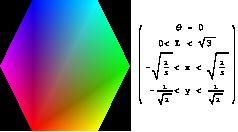
\includegraphics[width=0.49\textwidth]{Chapter3/Figs/xy_Polygon.jpg}
    \caption{The projection along the L axis showing the chromatic space with a free rotational angle of 0.}  \label{fig:xyPolygon}
\end{figure}



\subsection{Removing Zeroes}\label{sec:RemovingZeroes}

The obvious idea is to find all the non-zero bins and fit an interpolating function between them. This will effectively remove the empty bin artifacts within the densely-packed region which is the distribution we're interested in. However, the empty bins outside the main distribution are not artifacts and are genuinely empty bins, so removing all the empty bins and then fitting the function joins together any outlying points or secondary distributions corresponding to regions such as the background. We therefore desire a method which will allow us to keep all the non-empty bins and the empty bins outside the main distribution, i.e. all the genuinely empty bins. To achieve this, we designed a Matlab routine which essentially paints a region around each non-zero point, marking it as part of the main distribution. It then takes all the unmarked regions and includes all the empty bins in those regions. So, the set of points which is all the non-empty bins and all the empty bins in the unmarked regions satisfies the requirement, and a simple interpolating function can easily be fitted to those points.

%<flow chart, maybe? Or maybe at the end; we'll see.>

\subsection{White-Out and Black-Out}\label{sec:WhiteOutBlackOut}

Naively collapsing the bins along the luminosity axis artificially skews the chromatic distribution along the axis which passed through the luminosity axis; this is easily explained due to white-out and black-out. As luminosity increases or decreases, it will eventually hit the edge of the cube. Having reached its numerical limit, the luminosity slides toward the corner of the cube, resulting in a white or black value.

To accommodate this, we collapse the bins excluding the bins which are clearly suffering from white-out and black-out. This could be done mathematically by taking the bin of the distribution which is furthest from the luminosity axis, and then finding the intersection with the RGB cube when this chromatic value is at its limits, just before it reaches the edge of the cube where it suffers from white-out or black-out. But it's a simple matter to look at the three projections of the 3D LCaCb bins and manually determine the limits for the valid region.

%<Insert white-out/black-out bins here>

\subsection{Removing the Background Distribution}\label{sec:RemovingBGDistribution}

Having removed the empty bin artifacts and compensated for white-out/black-out effects, the final step is to remove the bin counts of the bins which are associated with the background, thereby leaving a distribution which corresponds to chromatic skin values and which is artifact- and systematic-error-free. With the chromatic bins processed as they have been so far, it is clear that there is a distinct distribution for the skin and a distinct distribution for the background. However, a distribution for the background was produced earlier, compensating for the iPhone's pre-AP-layer processing. Background removal is automated using a Matlab function which will negate the bins from one sample set using the distribution found for a second sample set.

%<Graph showing the overlap of the background and a skin background sample set; briefly describe what that shows.>

\subsection{Results}\label{sec:Results}

We're trying to develop a skin model from the Humane project, which provides a set which spans all the different skin tones. Although these images are not captured using the iPhone camera and thus suffer from a white point which does not correspond with the iPhone's white point (at least at the AP layer), it does provide a sufficient statistical basis to determine a color space region which is spanned by human skin. However, because of the iPhone camera's characteristics after pre-processing and the fact that the application needs to respond to an individual's skin, the investigation of skin tone characteristics for individuals is necessary.

To that effect, we selected three individuals with different skin tones; ordering by pigmentation from dark to light, we will henceforth refer to these as subjects F, N and J. Statistics were collected for the three subjects using the procedure outlined previously in this section. A two-dimensional Gaussian was fitted to the distribution for each individual.

\begin{figure}[h!]
  \centering
    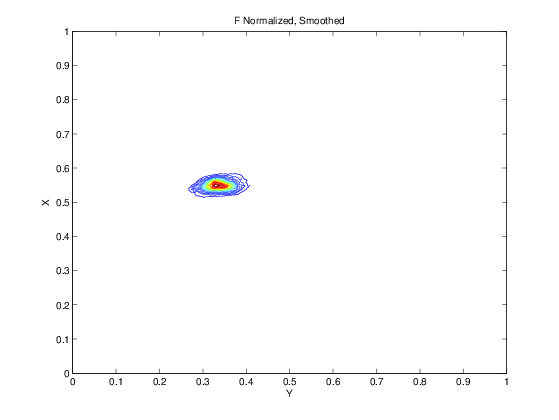
\includegraphics[width=0.49\textwidth]{Chapter3/Figs/FHands_XY_fBin.jpg}
    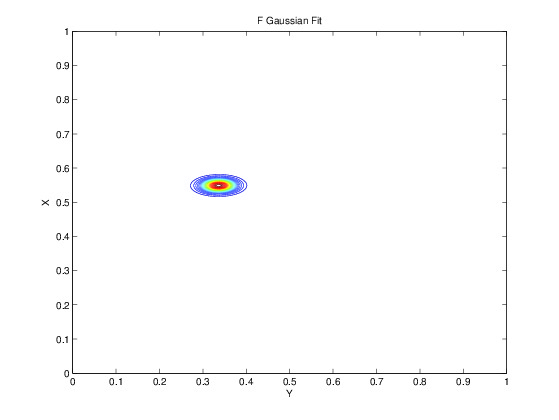
\includegraphics[width=0.49\textwidth]{Chapter3/Figs/FHands_XY_gFit.jpg}
    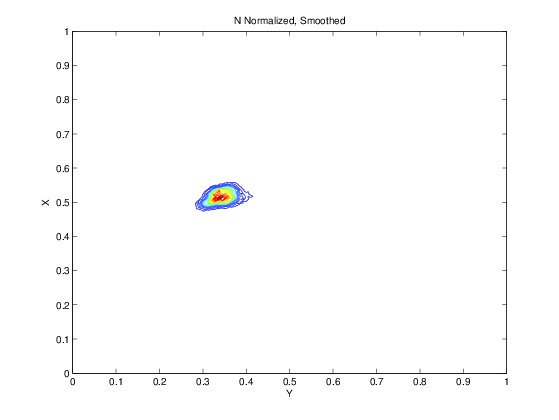
\includegraphics[width=0.49\textwidth]{Chapter3/Figs/NHands_XY_fBin.jpg}
    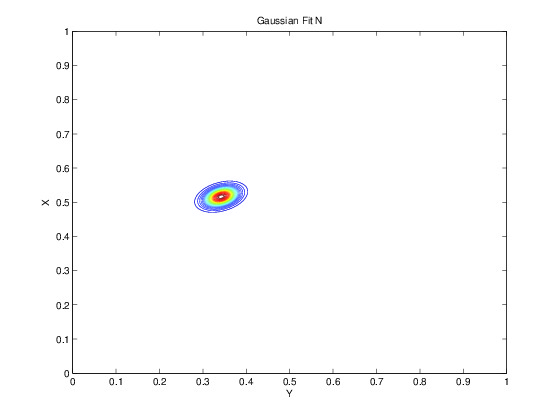
\includegraphics[width=0.49\textwidth]{Chapter3/Figs/NHands_XY_gFit.jpg}
    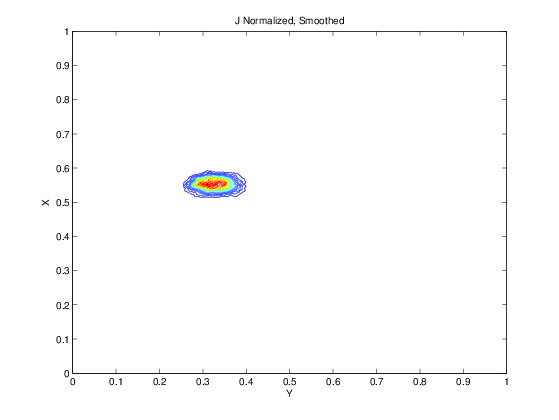
\includegraphics[width=0.49\textwidth]{Chapter3/Figs/JHands_XY_fBin.jpg}
    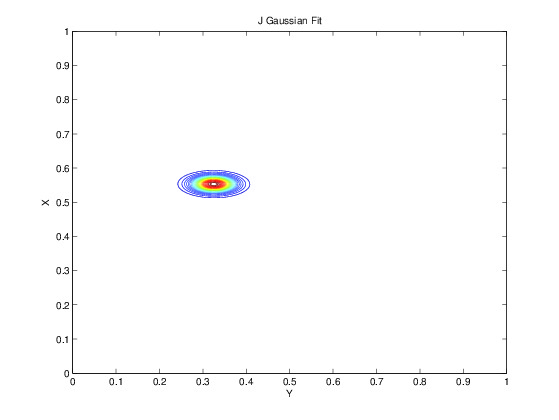
\includegraphics[width=0.49\textwidth]{Chapter3/Figs/JHands_XY_gFit.jpg}
    \caption{The CaCb bins after processing and the Gaussian fit.}  \label{fig:FBinAndGFit}
\end{figure}

The individual statistics are as follows:
\newline

\begin{tabular}{|c|c|c|c|c|c|c|}
\hline
& \multicolumn{2}{|c|}{Mean ($\mu$)} & \multicolumn{2}{|c|}{Standard Deviation ($\sigma$)} & \multicolumn{2}{|c|}{Angle ($\theta$)} \\\hline
& X & Y & X & Y & Major Axis & Minor Axis \\\hline
F & 0.4249 & 0.3335 & 0.0081 & 0.0251 & -0.7724 & 0.7984 \\\hline
N & 0.4281 & 0.3443 & 0.0080 & 0.0195 & -0.5549 & 0.5969 \\\hline
J & 0.4022 & 0.3302 & 0.0119 & 0.0253 & -0.8954 & 0.6754 \\\hline
\end{tabular}
\newline
\vspace{0.5 cm}
\newline
The statistics for the general sample set are as follows:
\newline

\begin{tabular}{|c|c|c|c|c|c|c|}
\hline
& \multicolumn{2}{|c|}{Mean ($\mu$)} & \multicolumn{2}{|c|}{Standard Deviation ($\sigma$)} & \multicolumn{2}{|c|}{Angle ($\theta$)} \\\hline
& X & Y & X & Y & Major Axis & Minor Axis \\\hline
General & 0.4820 & 0.4253 & 0.0072 & 0.0108 & -0.1174 & 1.4534 \\\hline
\end{tabular}



